% Options for packages loaded elsewhere
\PassOptionsToPackage{unicode}{hyperref}
\PassOptionsToPackage{hyphens}{url}
%
\documentclass[
]{article}
\usepackage{amsmath,amssymb}
\usepackage{iftex}
\ifPDFTeX
  \usepackage[T1]{fontenc}
  \usepackage[utf8]{inputenc}
  \usepackage{textcomp} % provide euro and other symbols
\else % if luatex or xetex
  \usepackage{unicode-math} % this also loads fontspec
  \defaultfontfeatures{Scale=MatchLowercase}
  \defaultfontfeatures[\rmfamily]{Ligatures=TeX,Scale=1}
\fi
\usepackage{lmodern}
\ifPDFTeX\else
  % xetex/luatex font selection
\fi
% Use upquote if available, for straight quotes in verbatim environments
\IfFileExists{upquote.sty}{\usepackage{upquote}}{}
\IfFileExists{microtype.sty}{% use microtype if available
  \usepackage[]{microtype}
  \UseMicrotypeSet[protrusion]{basicmath} % disable protrusion for tt fonts
}{}
\makeatletter
\@ifundefined{KOMAClassName}{% if non-KOMA class
  \IfFileExists{parskip.sty}{%
    \usepackage{parskip}
  }{% else
    \setlength{\parindent}{0pt}
    \setlength{\parskip}{6pt plus 2pt minus 1pt}}
}{% if KOMA class
  \KOMAoptions{parskip=half}}
\makeatother
\usepackage{xcolor}
\usepackage[margin=1in]{geometry}
\usepackage{color}
\usepackage{fancyvrb}
\newcommand{\VerbBar}{|}
\newcommand{\VERB}{\Verb[commandchars=\\\{\}]}
\DefineVerbatimEnvironment{Highlighting}{Verbatim}{commandchars=\\\{\}}
% Add ',fontsize=\small' for more characters per line
\usepackage{framed}
\definecolor{shadecolor}{RGB}{248,248,248}
\newenvironment{Shaded}{\begin{snugshade}}{\end{snugshade}}
\newcommand{\AlertTok}[1]{\textcolor[rgb]{0.94,0.16,0.16}{#1}}
\newcommand{\AnnotationTok}[1]{\textcolor[rgb]{0.56,0.35,0.01}{\textbf{\textit{#1}}}}
\newcommand{\AttributeTok}[1]{\textcolor[rgb]{0.13,0.29,0.53}{#1}}
\newcommand{\BaseNTok}[1]{\textcolor[rgb]{0.00,0.00,0.81}{#1}}
\newcommand{\BuiltInTok}[1]{#1}
\newcommand{\CharTok}[1]{\textcolor[rgb]{0.31,0.60,0.02}{#1}}
\newcommand{\CommentTok}[1]{\textcolor[rgb]{0.56,0.35,0.01}{\textit{#1}}}
\newcommand{\CommentVarTok}[1]{\textcolor[rgb]{0.56,0.35,0.01}{\textbf{\textit{#1}}}}
\newcommand{\ConstantTok}[1]{\textcolor[rgb]{0.56,0.35,0.01}{#1}}
\newcommand{\ControlFlowTok}[1]{\textcolor[rgb]{0.13,0.29,0.53}{\textbf{#1}}}
\newcommand{\DataTypeTok}[1]{\textcolor[rgb]{0.13,0.29,0.53}{#1}}
\newcommand{\DecValTok}[1]{\textcolor[rgb]{0.00,0.00,0.81}{#1}}
\newcommand{\DocumentationTok}[1]{\textcolor[rgb]{0.56,0.35,0.01}{\textbf{\textit{#1}}}}
\newcommand{\ErrorTok}[1]{\textcolor[rgb]{0.64,0.00,0.00}{\textbf{#1}}}
\newcommand{\ExtensionTok}[1]{#1}
\newcommand{\FloatTok}[1]{\textcolor[rgb]{0.00,0.00,0.81}{#1}}
\newcommand{\FunctionTok}[1]{\textcolor[rgb]{0.13,0.29,0.53}{\textbf{#1}}}
\newcommand{\ImportTok}[1]{#1}
\newcommand{\InformationTok}[1]{\textcolor[rgb]{0.56,0.35,0.01}{\textbf{\textit{#1}}}}
\newcommand{\KeywordTok}[1]{\textcolor[rgb]{0.13,0.29,0.53}{\textbf{#1}}}
\newcommand{\NormalTok}[1]{#1}
\newcommand{\OperatorTok}[1]{\textcolor[rgb]{0.81,0.36,0.00}{\textbf{#1}}}
\newcommand{\OtherTok}[1]{\textcolor[rgb]{0.56,0.35,0.01}{#1}}
\newcommand{\PreprocessorTok}[1]{\textcolor[rgb]{0.56,0.35,0.01}{\textit{#1}}}
\newcommand{\RegionMarkerTok}[1]{#1}
\newcommand{\SpecialCharTok}[1]{\textcolor[rgb]{0.81,0.36,0.00}{\textbf{#1}}}
\newcommand{\SpecialStringTok}[1]{\textcolor[rgb]{0.31,0.60,0.02}{#1}}
\newcommand{\StringTok}[1]{\textcolor[rgb]{0.31,0.60,0.02}{#1}}
\newcommand{\VariableTok}[1]{\textcolor[rgb]{0.00,0.00,0.00}{#1}}
\newcommand{\VerbatimStringTok}[1]{\textcolor[rgb]{0.31,0.60,0.02}{#1}}
\newcommand{\WarningTok}[1]{\textcolor[rgb]{0.56,0.35,0.01}{\textbf{\textit{#1}}}}
\usepackage{longtable,booktabs,array}
\usepackage{calc} % for calculating minipage widths
% Correct order of tables after \paragraph or \subparagraph
\usepackage{etoolbox}
\makeatletter
\patchcmd\longtable{\par}{\if@noskipsec\mbox{}\fi\par}{}{}
\makeatother
% Allow footnotes in longtable head/foot
\IfFileExists{footnotehyper.sty}{\usepackage{footnotehyper}}{\usepackage{footnote}}
\makesavenoteenv{longtable}
\usepackage{graphicx}
\makeatletter
\def\maxwidth{\ifdim\Gin@nat@width>\linewidth\linewidth\else\Gin@nat@width\fi}
\def\maxheight{\ifdim\Gin@nat@height>\textheight\textheight\else\Gin@nat@height\fi}
\makeatother
% Scale images if necessary, so that they will not overflow the page
% margins by default, and it is still possible to overwrite the defaults
% using explicit options in \includegraphics[width, height, ...]{}
\setkeys{Gin}{width=\maxwidth,height=\maxheight,keepaspectratio}
% Set default figure placement to htbp
\makeatletter
\def\fps@figure{htbp}
\makeatother
\setlength{\emergencystretch}{3em} % prevent overfull lines
\providecommand{\tightlist}{%
  \setlength{\itemsep}{0pt}\setlength{\parskip}{0pt}}
\setcounter{secnumdepth}{-\maxdimen} % remove section numbering
\usepackage{lipsum} \usepackage{float} \floatplacement{figure}{H}

\ifLuaTeX
  \usepackage{selnolig}  % disable illegal ligatures
\fi
\IfFileExists{bookmark.sty}{\usepackage{bookmark}}{\usepackage{hyperref}}
\IfFileExists{xurl.sty}{\usepackage{xurl}}{} % add URL line breaks if available
\urlstyle{same}
\hypersetup{
  pdftitle={Selection pressures in Syngnathus floridae},
  pdfauthor={Coley Tosto},
  hidelinks,
  pdfcreator={LaTeX via pandoc}}

\title{Selection pressures in \emph{Syngnathus floridae}}
\author{Coley Tosto}
\date{2023-11-08}

\begin{document}
\maketitle

\begin{Shaded}
\begin{Highlighting}[]
\CommentTok{\#This is a cohesive list of all the libraries used in this document}
\end{Highlighting}
\end{Shaded}

\begin{Shaded}
\begin{Highlighting}[]
\CommentTok{\#MomIDs and embryo counts for each section of the male\textquotesingle{}s brood pouch}
\NormalTok{em\_dat }\OtherTok{\textless{}{-}} \FunctionTok{read.csv}\NormalTok{(}\StringTok{"data/EmbryoParentage.csv"}\NormalTok{)}

\CommentTok{\#Metadata for males and females from the mesocosm experiments}
\NormalTok{fem\_meso }\OtherTok{\textless{}{-}} \FunctionTok{read.csv}\NormalTok{(}\StringTok{"data/all\_fem\_meso\_floridae.csv"}\NormalTok{)}
\NormalTok{mal\_meso }\OtherTok{\textless{}{-}} \FunctionTok{read.csv}\NormalTok{(}\StringTok{"data/all\_mal\_meso\_floridae.csv"}\NormalTok{)}
\end{Highlighting}
\end{Shaded}

\hypertarget{calculating-mating-and-reproductive-success-for-individuals-who-mated}{%
\section{Calculating mating and reproductive success for individuals who mated}\label{calculating-mating-and-reproductive-success-for-individuals-who-mated}}

\emph{Syngnathus floridae} (dusky pipefish) were sampled from three distinct seagrass beds around Tampa Bay in Tampa, Florida. Sexually mature females (standard length \(\ge\) 120mm) and pregnant males were collected and brought back to the University of Tampa for mesocosm experiments. In these mesocosms, 8 males and 8 females were housed together in a 140L tank for a period of 14-days and allowed to mate freely. Parentage analysis was done with all of the pregnant males from the trials to figure out how many times each male and female mated, and the number of eggs that were transferred. The results of that are here.

First I had to calculate the mating and reproductive success for each male and female who mated based on the assigned mom for each genotyped embryo.

\begin{Shaded}
\begin{Highlighting}[]
\CommentTok{\#Row{-}by{-}Row analysis of parentage data by male brood pouch section}

\CommentTok{\#Read in the data}
\CommentTok{\#em\_dat \textless{}{-} read.csv("\textasciitilde{}/EmbryoParentage.csv")}

\CommentTok{\#For each row in the dataset(each section of the pouch) apply this function}
\NormalTok{mom\_counts }\OtherTok{\textless{}{-}} \FunctionTok{do.call}\NormalTok{(rbind,}\FunctionTok{apply}\NormalTok{(em\_dat, }\DecValTok{1}\NormalTok{, }\ControlFlowTok{function}\NormalTok{(one\_section)\{}
  
  \CommentTok{\#Save all of the momIDs into an object}
\NormalTok{  mom\_ids}\OtherTok{\textless{}{-}}\FunctionTok{c}\NormalTok{(one\_section[}\FunctionTok{grep}\NormalTok{(}\StringTok{"momID"}\NormalTok{,}\FunctionTok{names}\NormalTok{(one\_section))])  }
  
  \CommentTok{\#Calculate the number of eggs that belongs to each potential mom based on}
  \CommentTok{\#the proportions and total number of developed and undeveloped embryos}
\NormalTok{  mom\_props}\OtherTok{\textless{}{-}}\FunctionTok{c}\NormalTok{(}\FunctionTok{as.numeric}\NormalTok{(one\_section[}\FunctionTok{grep}\NormalTok{(}\StringTok{"prop"}\NormalTok{,}\FunctionTok{names}\NormalTok{(one\_section))]))}
\NormalTok{  mom\_counts\_dev}\OtherTok{\textless{}{-}}\NormalTok{mom\_props}\SpecialCharTok{*}\FunctionTok{as.numeric}\NormalTok{(one\_section[}\StringTok{"num\_embryos\_dev"}\NormalTok{])}
\NormalTok{  mom\_counts\_und}\OtherTok{\textless{}{-}}\NormalTok{mom\_props}\SpecialCharTok{*}\FunctionTok{as.numeric}\NormalTok{(one\_section[}\StringTok{"num\_embryos\_non\_dev"}\NormalTok{])}
  
  \CommentTok{\#Create a dataframe that contains the maleID, pouch section number and the}
  \CommentTok{\#number of eggs that belongs to each momID}
\NormalTok{  this\_section}\OtherTok{\textless{}{-}}\FunctionTok{data.frame}\NormalTok{(}
    \AttributeTok{maleID=}\NormalTok{one\_section[}\StringTok{"maleID"}\NormalTok{],}
    \AttributeTok{section\_num=}\NormalTok{one\_section[}\StringTok{"section\_num"}\NormalTok{],}
\NormalTok{    mom\_ids[}\FunctionTok{which}\NormalTok{((mom\_counts\_dev }\SpecialCharTok{+}\NormalTok{ mom\_counts\_und) }\SpecialCharTok{\textgreater{}} \DecValTok{0}\NormalTok{)],}
\NormalTok{    mom\_counts\_dev[}\FunctionTok{which}\NormalTok{((mom\_counts\_dev }\SpecialCharTok{+}\NormalTok{ mom\_counts\_und)}\SpecialCharTok{\textgreater{}}\DecValTok{0}\NormalTok{)],}
\NormalTok{    mom\_counts\_und[}\FunctionTok{which}\NormalTok{((mom\_counts\_dev }\SpecialCharTok{+}\NormalTok{ mom\_counts\_und)}\SpecialCharTok{\textgreater{}}\DecValTok{0}\NormalTok{)]}
\NormalTok{  )}
  
  \CommentTok{\#Rename the columns}
  \FunctionTok{colnames}\NormalTok{(this\_section)[}\DecValTok{3}\SpecialCharTok{:}\DecValTok{5}\NormalTok{]}\OtherTok{\textless{}{-}}\FunctionTok{c}\NormalTok{(}\StringTok{"momID"}\NormalTok{,}\StringTok{"num\_dev"}\NormalTok{,}\StringTok{"num\_und"}\NormalTok{)}
  
  \FunctionTok{return}\NormalTok{(this\_section)}
  
\NormalTok{\}))}

\CommentTok{\#Calculate female fitness}
\NormalTok{fem\_fitness}\OtherTok{\textless{}{-}}\FunctionTok{do.call}\NormalTok{(rbind,}\FunctionTok{by}\NormalTok{(mom\_counts, mom\_counts}\SpecialCharTok{$}\NormalTok{momID,}\ControlFlowTok{function}\NormalTok{(dat)\{}
  
\NormalTok{  mom\_fitness}\OtherTok{\textless{}{-}}\FunctionTok{data.frame}\NormalTok{(}
    \AttributeTok{momID=}\FunctionTok{unique}\NormalTok{(dat}\SpecialCharTok{$}\NormalTok{momID),}
    \AttributeTok{MatingSuccess=}\FunctionTok{length}\NormalTok{(}\FunctionTok{unique}\NormalTok{(dat}\SpecialCharTok{$}\NormalTok{maleID)),}
    \AttributeTok{NumDeveloped=}\FunctionTok{round}\NormalTok{(}\FunctionTok{sum}\NormalTok{(dat}\SpecialCharTok{$}\NormalTok{num\_dev)),}
    \AttributeTok{NumUndeveloped=}\FunctionTok{round}\NormalTok{(}\FunctionTok{sum}\NormalTok{(dat}\SpecialCharTok{$}\NormalTok{num\_und))}
\NormalTok{  )}
  \FunctionTok{return}\NormalTok{(mom\_fitness)}
\NormalTok{\}))}

\NormalTok{fem\_fitness}\SpecialCharTok{$}\NormalTok{totalEggs }\OtherTok{\textless{}{-}}\NormalTok{ fem\_fitness}\SpecialCharTok{$}\NormalTok{NumDeveloped }\SpecialCharTok{+}\NormalTok{ fem\_fitness}\SpecialCharTok{$}\NormalTok{NumUndeveloped}

\CommentTok{\#Calculate Male Fitness }
\NormalTok{mal\_fitness}\OtherTok{\textless{}{-}}\FunctionTok{do.call}\NormalTok{(rbind,}\FunctionTok{by}\NormalTok{(mom\_counts, mom\_counts}\SpecialCharTok{$}\NormalTok{maleID,}\ControlFlowTok{function}\NormalTok{(dat)\{}
 
\NormalTok{  dad\_fitness}\OtherTok{\textless{}{-}}\FunctionTok{data.frame}\NormalTok{(}
    \AttributeTok{maleID=}\FunctionTok{unique}\NormalTok{(dat}\SpecialCharTok{$}\NormalTok{maleID),}
    \AttributeTok{MatingSuccess=}\FunctionTok{length}\NormalTok{(}\FunctionTok{unique}\NormalTok{(dat}\SpecialCharTok{$}\NormalTok{momID)),}
    \AttributeTok{NumDeveloped\_Calc=}\FunctionTok{round}\NormalTok{(}\FunctionTok{sum}\NormalTok{(dat}\SpecialCharTok{$}\NormalTok{num\_dev)),}
    \AttributeTok{NumUndeveloped\_Calc=}\FunctionTok{round}\NormalTok{(}\FunctionTok{sum}\NormalTok{(dat}\SpecialCharTok{$}\NormalTok{num\_und))}
\NormalTok{  )}
  \FunctionTok{return}\NormalTok{(dad\_fitness)}
\NormalTok{\}))}

\NormalTok{mal\_fitness}\SpecialCharTok{$}\NormalTok{totalEggs }\OtherTok{\textless{}{-}}\NormalTok{ mal\_fitness}\SpecialCharTok{$}\NormalTok{NumDeveloped\_Calc }\SpecialCharTok{+}\NormalTok{ mal\_fitness}\SpecialCharTok{$}\NormalTok{NumUndeveloped\_Calc}
\end{Highlighting}
\end{Shaded}

After running the above R script we have two datasets, \texttt{mal\_fitness} and \texttt{fem\_fitness}. These datasets include information about the mating success (number of mates) and reproductive success (Number of embryos transferred). We can split reproductive success up further later if we want to from the total number of embryos transferred to the number of embryos developed and the number that were undeveloped.

I want to include all of the other metadata that I have for these individuals (traits, collection location, latency to pregnancy, etc.) as well as tack on all of the information for the individuals who did not mate. To do that I am going to need to merge the fitness datasets with \texttt{fem\_meso} and \texttt{mal\_meso}.

\begin{Shaded}
\begin{Highlighting}[]
\CommentTok{\#Make a column in *\_meso that contains the full fishID (i.e. FL1M3) to match the }
\CommentTok{\#formatting in the fitness datasets (make sure they have the same name for merging purposes)}
\NormalTok{fem\_meso}\SpecialCharTok{$}\NormalTok{momID }\OtherTok{\textless{}{-}} \FunctionTok{paste0}\NormalTok{(}\StringTok{"FL"}\NormalTok{, fem\_meso}\SpecialCharTok{$}\NormalTok{trial\_num, }\StringTok{"F"}\NormalTok{, fem\_meso}\SpecialCharTok{$}\NormalTok{fishID)}
\NormalTok{mal\_meso}\SpecialCharTok{$}\NormalTok{maleID }\OtherTok{\textless{}{-}} \FunctionTok{paste0}\NormalTok{(}\StringTok{"FL"}\NormalTok{, mal\_meso}\SpecialCharTok{$}\NormalTok{trial\_num, }\StringTok{"M"}\NormalTok{, mal\_meso}\SpecialCharTok{$}\NormalTok{fishID)}

\CommentTok{\#Merge the datasets based on the columns created above}
\NormalTok{fem\_all }\OtherTok{\textless{}{-}} \FunctionTok{merge}\NormalTok{(fem\_meso, fem\_fitness, }\AttributeTok{by =} \StringTok{"momID"}\NormalTok{, }\AttributeTok{all.x =} \ConstantTok{TRUE}\NormalTok{, }\AttributeTok{all.y =} \ConstantTok{TRUE}\NormalTok{)}
\NormalTok{mal\_all }\OtherTok{\textless{}{-}} \FunctionTok{merge}\NormalTok{(mal\_meso, mal\_fitness, }\AttributeTok{by =} \StringTok{"maleID"}\NormalTok{, }\AttributeTok{all.x =} \ConstantTok{TRUE}\NormalTok{, }\AttributeTok{all.y =} \ConstantTok{TRUE}\NormalTok{)}
\end{Highlighting}
\end{Shaded}

There are a few trials that I want to remove from the analysis:

\begin{enumerate}
\def\labelenumi{\arabic{enumi}.}
\item
  All trials where there were no successful matings (7, 9, 10, 11).
\item
  Trial 1, a male gave birth and the babies were immediately eaten by the adults so the trial was ended early and therefore I was unable to get any parentage information for that trial.
\end{enumerate}

I also want to replace the NAs that were automatically added to the columns from the fitness dataset (MatingSuccess, NumDeveloped, NumUndeveloped, totalEggs) with 0s and add a column to the female dataset that tells me whether or not the female mated (with 1 or 0).

\begin{Shaded}
\begin{Highlighting}[]
\CommentTok{\#Subset the merged datasets to remove trials without successful matings and Trial 1}
\NormalTok{fem\_succ }\OtherTok{\textless{}{-}} \FunctionTok{subset}\NormalTok{(fem\_all, }\SpecialCharTok{!}\NormalTok{(trial\_num }\SpecialCharTok{\%in\%} \FunctionTok{c}\NormalTok{(}\DecValTok{7}\NormalTok{, }\DecValTok{9}\NormalTok{, }\DecValTok{10}\NormalTok{, }\DecValTok{11}\NormalTok{, }\DecValTok{1}\NormalTok{)))}
\NormalTok{mal\_succ }\OtherTok{\textless{}{-}} \FunctionTok{subset}\NormalTok{(mal\_all, }\SpecialCharTok{!}\NormalTok{(trial\_num }\SpecialCharTok{\%in\%} \FunctionTok{c}\NormalTok{(}\DecValTok{7}\NormalTok{, }\DecValTok{9}\NormalTok{, }\DecValTok{10}\NormalTok{, }\DecValTok{11}\NormalTok{, }\DecValTok{1}\NormalTok{)))}

\CommentTok{\#Replace NAs with 0s in the columns related to fitness}
\NormalTok{mal\_succ[,}\DecValTok{15}\SpecialCharTok{:}\DecValTok{18}\NormalTok{] }\OtherTok{\textless{}{-}} \FunctionTok{sapply}\NormalTok{(mal\_succ[,}\DecValTok{15}\SpecialCharTok{:}\DecValTok{18}\NormalTok{],}
                           \ControlFlowTok{function}\NormalTok{(x)}
                             \FunctionTok{ifelse}\NormalTok{(}\FunctionTok{is.na}\NormalTok{(x), }\DecValTok{0}\NormalTok{, x))}

\NormalTok{fem\_succ[,}\DecValTok{11}\SpecialCharTok{:}\DecValTok{14}\NormalTok{] }\OtherTok{\textless{}{-}} \FunctionTok{sapply}\NormalTok{(fem\_succ[,}\DecValTok{11}\SpecialCharTok{:}\DecValTok{14}\NormalTok{],}
                           \ControlFlowTok{function}\NormalTok{(x)}
                             \FunctionTok{ifelse}\NormalTok{(}\FunctionTok{is.na}\NormalTok{(x), }\DecValTok{0}\NormalTok{, x))}

\CommentTok{\#Add a column for females to denote mated or unmated}
\NormalTok{fem\_succ}\SpecialCharTok{$}\NormalTok{mated }\OtherTok{\textless{}{-}} \FunctionTok{ifelse}\NormalTok{(fem\_succ}\SpecialCharTok{$}\NormalTok{MatingSuccess }\SpecialCharTok{\textgreater{}} \DecValTok{0}\NormalTok{, }\FunctionTok{paste0}\NormalTok{(}\DecValTok{1}\NormalTok{), }\FunctionTok{paste0}\NormalTok{(}\DecValTok{0}\NormalTok{))}
\end{Highlighting}
\end{Shaded}

\hypertarget{summary-statistics-for-successfully-mated-individuals}{%
\section{Summary statistics for successfully mated individuals}\label{summary-statistics-for-successfully-mated-individuals}}

\hypertarget{males}{%
\subsection{Males}\label{males}}

Across all 7 trials and 56 total males, there were 22 males that mated at least one time and 6 of those males had two mates.

Looking across all males, including the ones that did not mate, this is what we find as the mean, sd, and se for the number of embryos transferred and how many of those developed versus didn't:

\begin{longtable}[]{@{}lrrrrr@{}}
\toprule\noalign{}
& mean & SD & SE & max & min \\
\midrule\noalign{}
\endhead
\bottomrule\noalign{}
\endlastfoot
Number of Embryos & 108.5 & 155.1902059 & 20.7381636 & 500 & 0 \\
Developed Embryos & 94.1964286 & 139.7347383 & 18.6728398 & 463 & 0 \\
Undeveloped Embryos & 14.3035714 & 27.7907242 & 3.7136917 & 131 & 0 \\
\end{longtable}

These values will be influenced by the number of 0s coming from males who did not mate. So let's look at the same thing, but this time for only males who had at least one successful mating:

\begin{longtable}[]{@{}lrrrrr@{}}
\toprule\noalign{}
& mean & SD & SE & max & min \\
\midrule\noalign{}
\endhead
\bottomrule\noalign{}
\endlastfoot
Number of Embryos & 271.0454545 & 130.7948147 & 27.8855482 & 500 & 9 \\
Developed Embryos & 234.7727273 & 129.1646907 & 27.5380046 & 463 & 7 \\
Undeveloped Embryos & 36.2727273 & 34.4897249 & 7.3532341 & 131 & 0 \\
\end{longtable}

We can see from the bottom table that even when we only include males who mated there is still a wide range in the brood size. I want to see what relationship there is between brood pouch size (in terms of both total area and length) and brood size (total number of embryos).

\begin{figure}
\centering
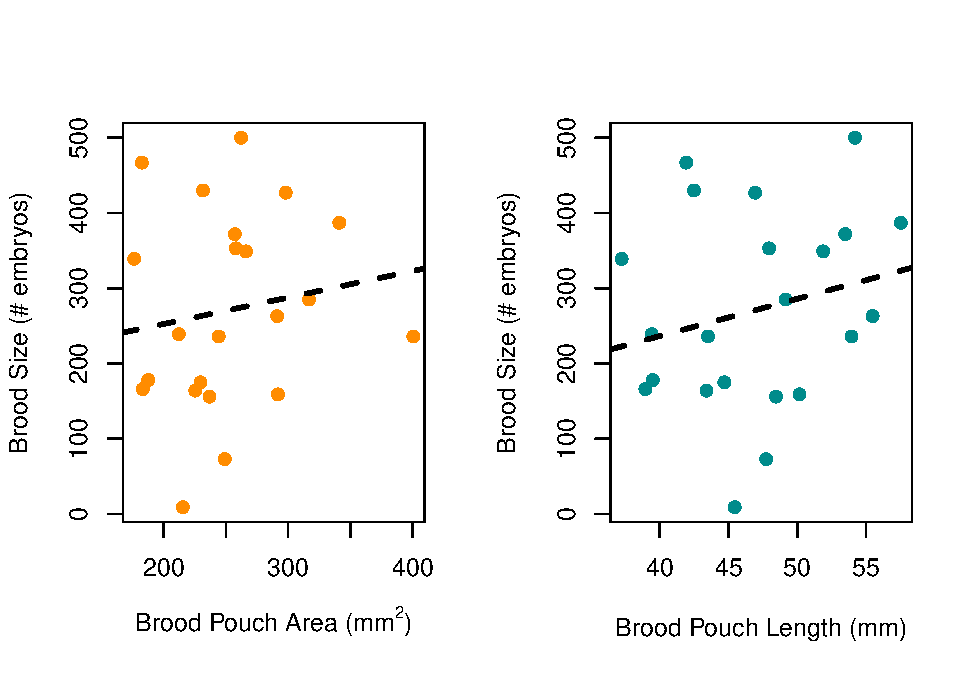
\includegraphics{selection_analysis_floridae_files/figure-latex/em-v-bp-1.pdf}
\caption{\label{fig:em-v-bp}Scatterplot of the relationship between brood pouch size metrics and the number of embryos a male had.}
\end{figure}

There may be some correlation happening here, but it doesn't look particularly strong (Fig. \ref{fig:em-v-bp}). Let's run some correlations tests to see what they say.

\begin{verbatim}
## 
##  Pearson's product-moment correlation
## 
## data:  as.numeric(mated_mal$bp_area) and mated_mal$totalEggs
## t = 0.6717, df = 20, p-value = 0.5095
## alternative hypothesis: true correlation is not equal to 0
## 95 percent confidence interval:
##  -0.2913214  0.5365395
## sample estimates:
##     cor 
## 0.14853
\end{verbatim}

\begin{verbatim}
## 
##  Pearson's product-moment correlation
## 
## data:  as.numeric(mated_mal$bp_length) and mated_mal$totalEggs
## t = 1.0182, df = 20, p-value = 0.3208
## alternative hypothesis: true correlation is not equal to 0
## 95 percent confidence interval:
##  -0.2202318  0.5885165
## sample estimates:
##       cor 
## 0.2219886
\end{verbatim}

There is not a significant correlation between the number of eggs and size of the brood pouch when we look at brood pouch area OR brood pouch length.

\hypertarget{females}{%
\subsection{Females}\label{females}}

Across all 7 trials and 56 total females, there were 21 females that mated at least one time, 5 females that mated twice, and 2 that mated 3 times.

Looking across all females, including the ones that did not mate, this is what we find as the mean, sd, and se for the total number of embryos transferred from each female (across all of her mates if applicable) and how many of those developed versus didn't:

\begin{longtable}[]{@{}lrrrrr@{}}
\toprule\noalign{}
& mean & SD & SE & max & min \\
\midrule\noalign{}
\endhead
\bottomrule\noalign{}
\endlastfoot
Number of Embryos & 108.4821429 & 195.2328206 & 26.089083 & 916 & 0 \\
Developed Embryos & 94.1785714 & 177.0691808 & 23.6618646 & 785 & 0 \\
Undeveloped Embryos & 14.3035714 & 29.7033329 & 3.9692748 & 131 & 0 \\
\end{longtable}

These values will be influenced by the number of 0s coming from females who did not mate. So let's look at the same thing, but this time for only females who had at least one successful mating:

\begin{longtable}[]{@{}lrrrrr@{}}
\toprule\noalign{}
& mean & SD & SE & max & min \\
\midrule\noalign{}
\endhead
\bottomrule\noalign{}
\endlastfoot
Number of Embryos & 289.2857143 & 223.3819919 & 48.745947 & 916 & 35 \\
Developed Embryos & 251.1428571 & 211.7324457 & 46.2038076 & 785 & 7 \\
Undeveloped Embryos & 38.1428571 & 38.360508 & 8.3709491 & 131 & 0 \\
\end{longtable}

We can see from the bottom table that even when we only include females who mated there is still a wide range in the number of eggs transferred. I want to see what relationship there may be between female body size (in terms of standard length, depth, and SVL) and the number of eggs she transferred.

\begin{figure}
\centering
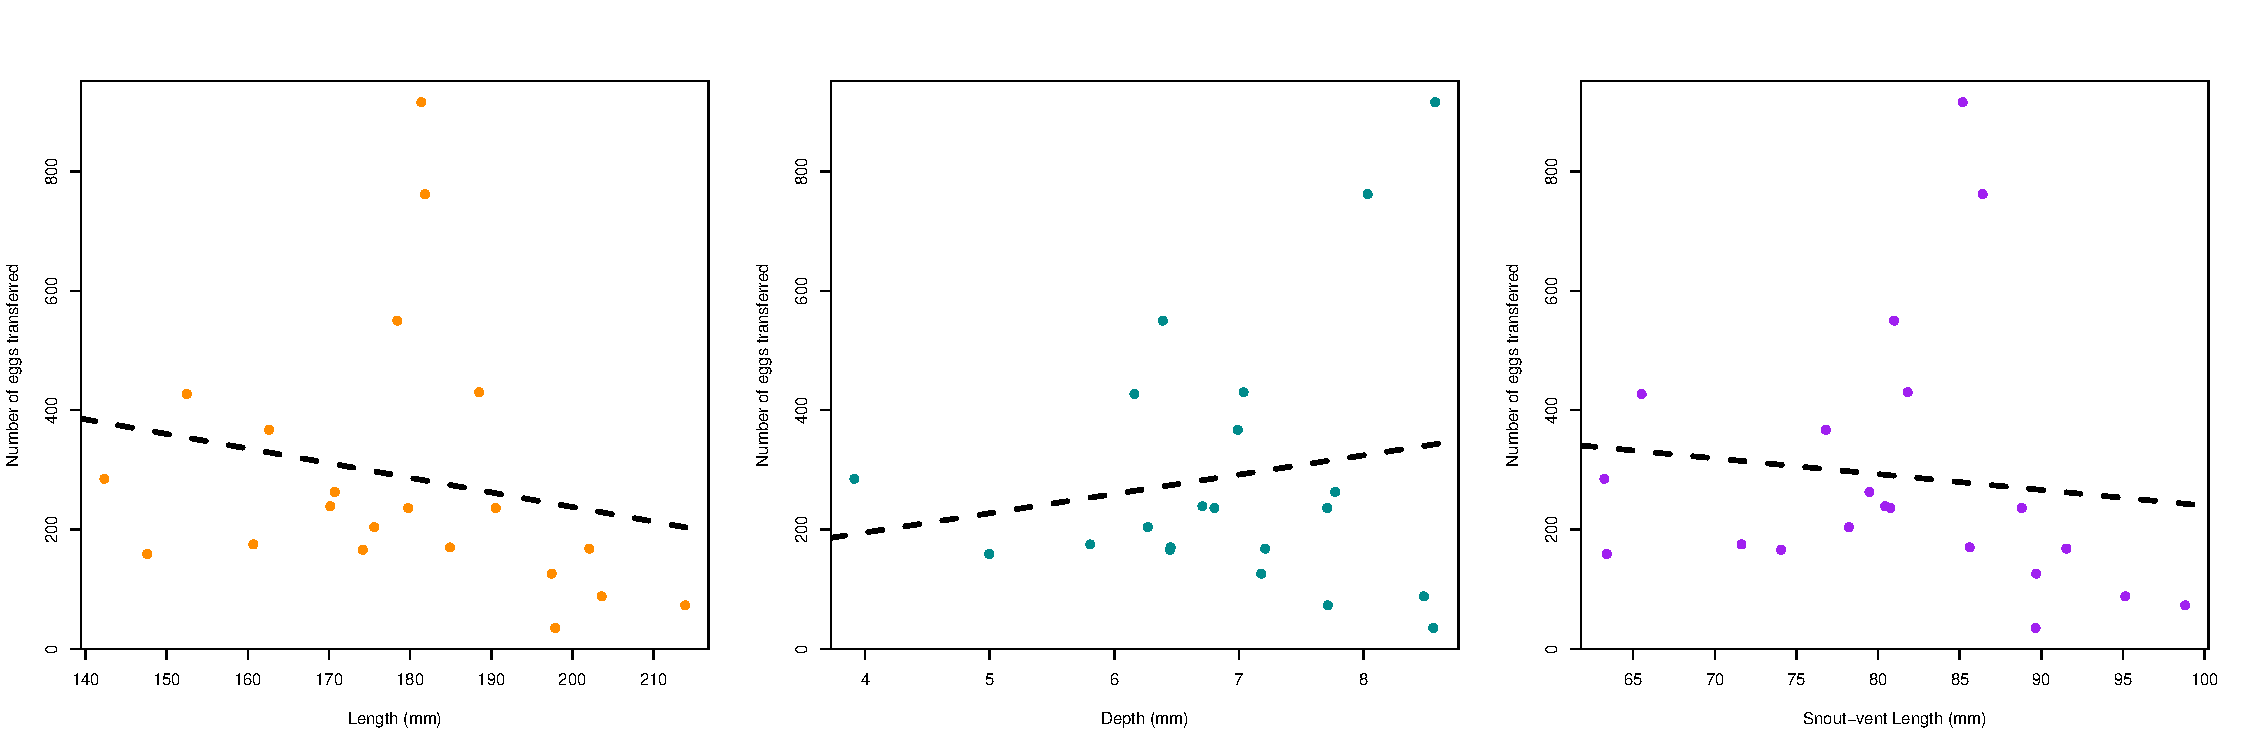
\includegraphics{selection_analysis_floridae_files/figure-latex/em-v-fem-size-1.pdf}
\caption{\label{fig:em-v-fem-size}Scatterplot of the relationship between female size metrics and the number of eggs transferred.}
\end{figure}

There may be some correlation happening here, but it doesn't look particularly strong (Fig. \ref{fig:em-v-fem-size}). Let's run some correlations tests to see what they say.

\begin{verbatim}
## 
##  Pearson's product-moment correlation
## 
## data:  mated_fem$length and as.numeric(mated_fem$totalEggs)
## t = -0.92304, df = 19, p-value = 0.3676
## alternative hypothesis: true correlation is not equal to 0
## 95 percent confidence interval:
##  -0.5864091  0.2465727
## sample estimates:
##        cor 
## -0.2071652
\end{verbatim}

\begin{verbatim}
## 
##  Pearson's product-moment correlation
## 
## data:  mated_fem$depth and as.numeric(mated_fem$totalEggs)
## t = 0.74454, df = 19, p-value = 0.4657
## alternative hypothesis: true correlation is not equal to 0
## 95 percent confidence interval:
##  -0.2839543  0.5593989
## sample estimates:
##       cor 
## 0.1683713
\end{verbatim}

\begin{verbatim}
## 
##  Pearson's product-moment correlation
## 
## data:  mated_fem$svl and as.numeric(mated_fem$totalEggs)
## t = -0.5112, df = 19, p-value = 0.6151
## alternative hypothesis: true correlation is not equal to 0
## 95 percent confidence interval:
##  -0.5219227  0.3318958
## sample estimates:
##        cor 
## -0.1164796
\end{verbatim}

There is not a significant correlation between the number of eggs and size of the female in terms of standard length, depth, or snout-vent length. Interestingly, however, there is a negative correlation for length and SVL and a positive correlation for depth (but they are all overall weak).

\hypertarget{differences-between-mated-individuals-and-unmated-individuals}{%
\section{Differences between mated individuals and unmated individuals}\label{differences-between-mated-individuals-and-unmated-individuals}}

I want to now see if there are any significant differences in the sizes of individuals who mated vs individuals that didn't mate in males and females.

\hypertarget{males-1}{%
\subsection{Males}\label{males-1}}

\begin{figure}
\centering
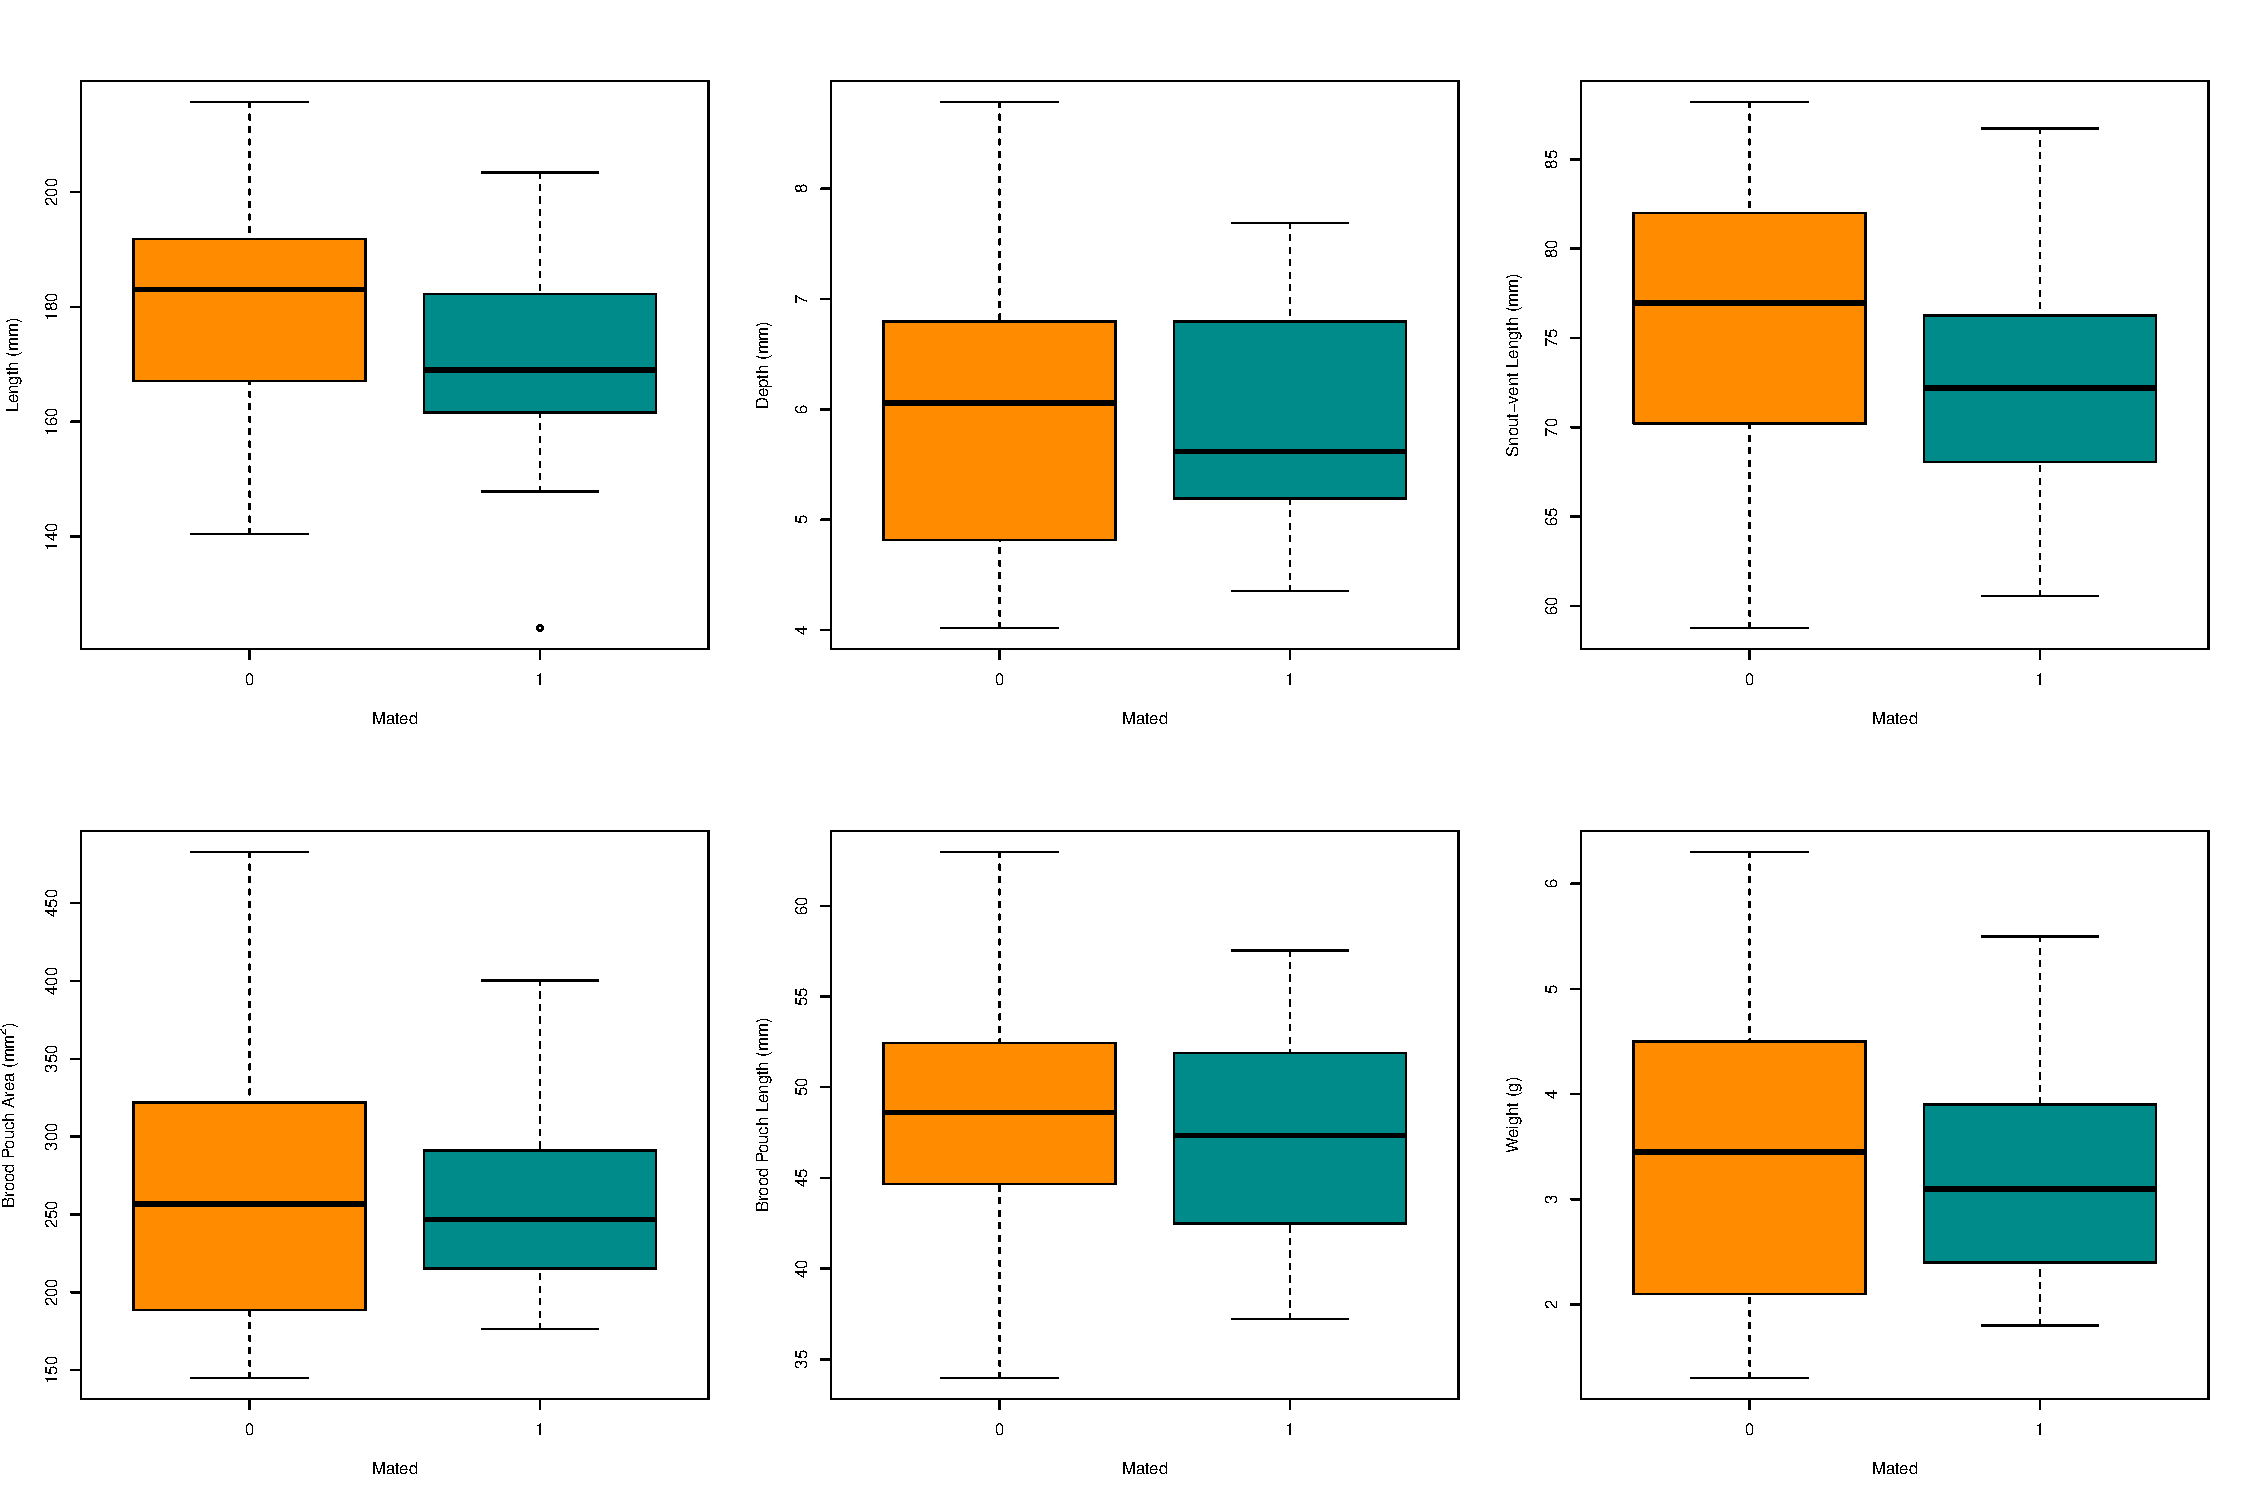
\includegraphics{selection_analysis_floridae_files/figure-latex/mat-status-morph-mal-1.pdf}
\caption{\label{fig:mat-status-morph-mal}Six different morphometrics compared between males who sucessfully mated versus those that didn't. Orange represents unmated and blue represents mated males.}
\end{figure}

\begin{verbatim}
## 
##  Wilcoxon rank sum exact test
## 
## data:  mal_succ$length by mal_succ$preg_status
## W = 463, p-value = 0.08745
## alternative hypothesis: true location shift is not equal to 0
\end{verbatim}

\begin{verbatim}
## 
##  Wilcoxon rank sum test with continuity correction
## 
## data:  mal_succ$depth by mal_succ$preg_status
## W = 362, p-value = 0.9931
## alternative hypothesis: true location shift is not equal to 0
\end{verbatim}

\begin{verbatim}
## 
##  Wilcoxon rank sum exact test
## 
## data:  mal_succ$svl by mal_succ$preg_status
## W = 472, p-value = 0.06194
## alternative hypothesis: true location shift is not equal to 0
\end{verbatim}

\begin{verbatim}
## 
##  Wilcoxon rank sum exact test
## 
## data:  as.numeric(mal_succ$bp_area) by mal_succ$preg_status
## W = 358, p-value = 0.7678
## alternative hypothesis: true location shift is not equal to 0
\end{verbatim}

\begin{verbatim}
## 
##  Wilcoxon rank sum exact test
## 
## data:  mal_succ$bp_length by mal_succ$preg_status
## W = 388, p-value = 0.4045
## alternative hypothesis: true location shift is not equal to 0
\end{verbatim}

\begin{verbatim}
## 
##  Wilcoxon rank sum test with continuity correction
## 
## data:  mal_succ$weight by mal_succ$preg_status
## W = 400, p-value = 0.6686
## alternative hypothesis: true location shift is not equal to 0
\end{verbatim}

\hypertarget{females-1}{%
\subsection{Females}\label{females-1}}

\begin{figure}
\centering
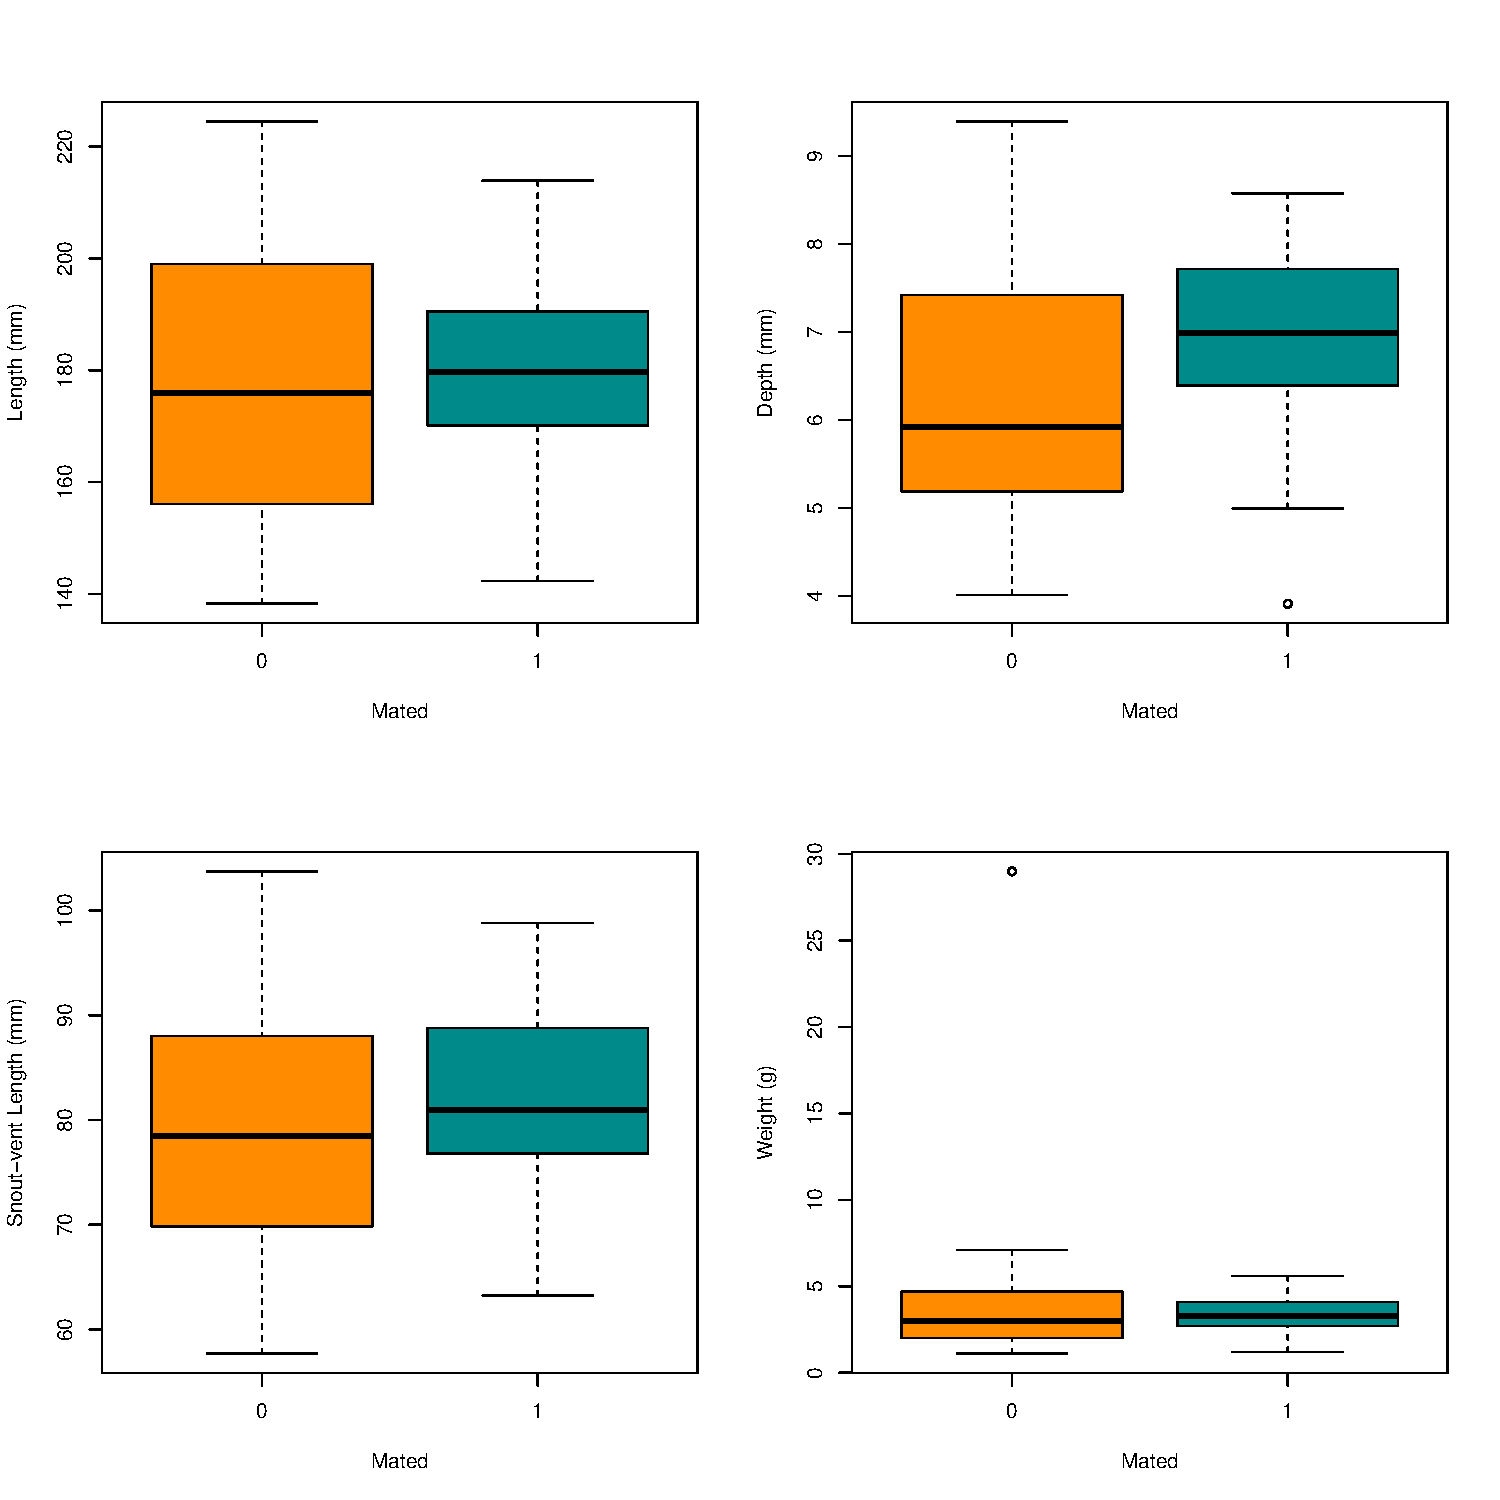
\includegraphics{selection_analysis_floridae_files/figure-latex/mat-status-morph-fem-1.pdf}
\caption{\label{fig:mat-status-morph-fem}Four different morphometrics compared between females who sucessfully mated versus those that didn't. Orange represents unmated and blue represents mated females.}
\end{figure}

\begin{verbatim}
## 
##  Wilcoxon rank sum exact test
## 
## data:  fem_succ$length by fem_succ$mated
## W = 353, p-value = 0.8143
## alternative hypothesis: true location shift is not equal to 0
\end{verbatim}

\begin{verbatim}
## 
##  Wilcoxon rank sum exact test
## 
## data:  fem_succ$depth by fem_succ$mated
## W = 261, p-value = 0.07263
## alternative hypothesis: true location shift is not equal to 0
\end{verbatim}

\begin{verbatim}
## 
##  Wilcoxon rank sum exact test
## 
## data:  fem_succ$svl by fem_succ$mated
## W = 325, p-value = 0.4805
## alternative hypothesis: true location shift is not equal to 0
\end{verbatim}

\begin{verbatim}
## 
##  Wilcoxon rank sum test with continuity correction
## 
## data:  fem_succ$weight by fem_succ$mated
## W = 338.5, p-value = 0.6292
## alternative hypothesis: true location shift is not equal to 0
\end{verbatim}

\hypertarget{mate-success-versus-reproductive-success}{%
\section{Mate success versus Reproductive success}\label{mate-success-versus-reproductive-success}}

I now want to look at any relationship that may exist between mating success and reproductive success for males and females. The Bateman gradient will be calculated, which is the slope of the weighted least-squares regression of relative reproductive success (number of offspring divided by the mean) on mating success.

\begin{figure}
\centering
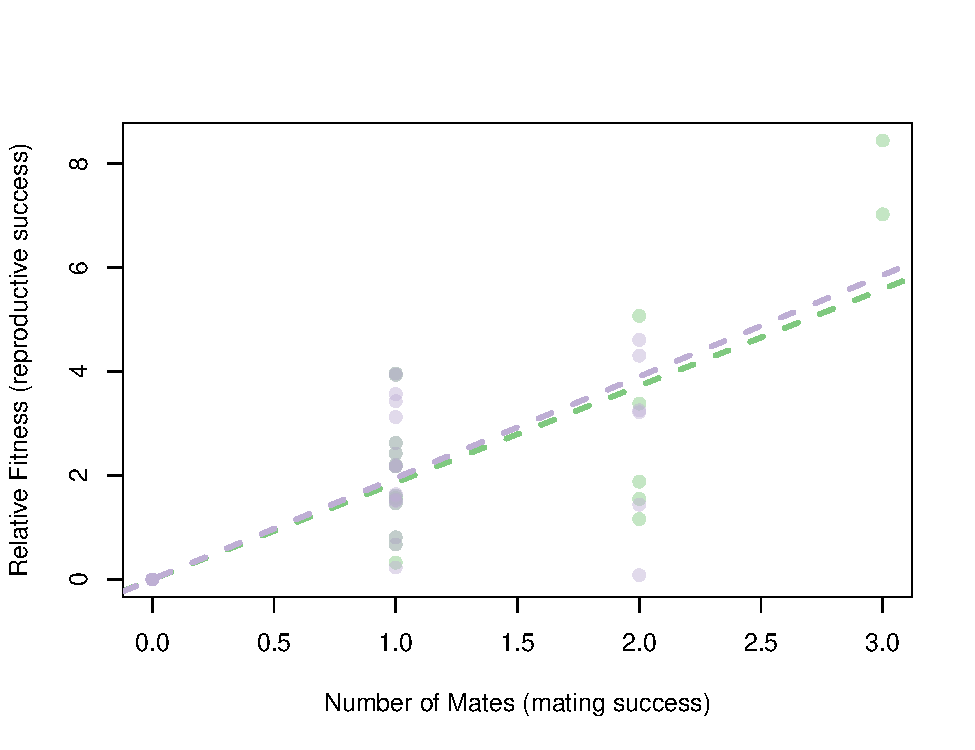
\includegraphics{selection_analysis_floridae_files/figure-latex/unnamed-chunk-1-1.pdf}
\caption{\label{fig:unnamed-chunk-1}Relationship between reproductive success and mating success for male (purple) and female (green) \emph{Syngnathus floridae}. Reproductive success is shown as relative fitness (i.e.~number of offspring produced divided by the mean number of offspring produced). Bateman's gradient is shown as the weighted least-squares regression line (dashed) for males and females.}
\end{figure}

\end{document}
